This section describes how typical GPUs work and how GPUs differ from other accelerator types.\par

\hspace*{\fill} \par %插入空行
\textbf{GPU Building Blocks}

Figure 15-1 shows a very simplified GPU consisting of three high-level building blocks:\par

\begin{itemize}
	\item Execution resources: A GPU’s execution resources are the processors that perform computational work. Different GPU vendors use different names for their execution resources, but all modern GPUs consist of multiple programmable processors. The processors may be heterogeneous and specialized for particular tasks, or they may be homogeneous and interchangeable. Processors for most modern GPUs are homogeneous and interchangeable.
	\item Fixed functions: GPU fixed functions are hardware units that are less programmable than the execution resources and are specialized for a single task. 
	When a GPU is used for graphics, many parts of the graphics pipeline such as rasterization or raytracing are performed using fixed functions to improve 
	power efficiency and performance. When a GPU is used for data-parallel computation, fixed functions may be used for tasks such as workload scheduling, 
	texture sampling, and dependence tracking.
	\item Caches and memory: Like other processor types, GPUs frequently have caches to store data accessed by the execution resources. GPU caches may be 
	implicit, in which case they require no action from the programmer, or may be explicit scratchpad memories, in which case a programmer must purposefully move data into a cache before using it. Many GPUs also have a large pool of memory to provide fast access to data used by the execution 
	resources.
\end{itemize}

\hspace*{\fill} \par %插入空行
Figure 15-1. Typical GPU building blocks—not to scale!
\begin{center}
	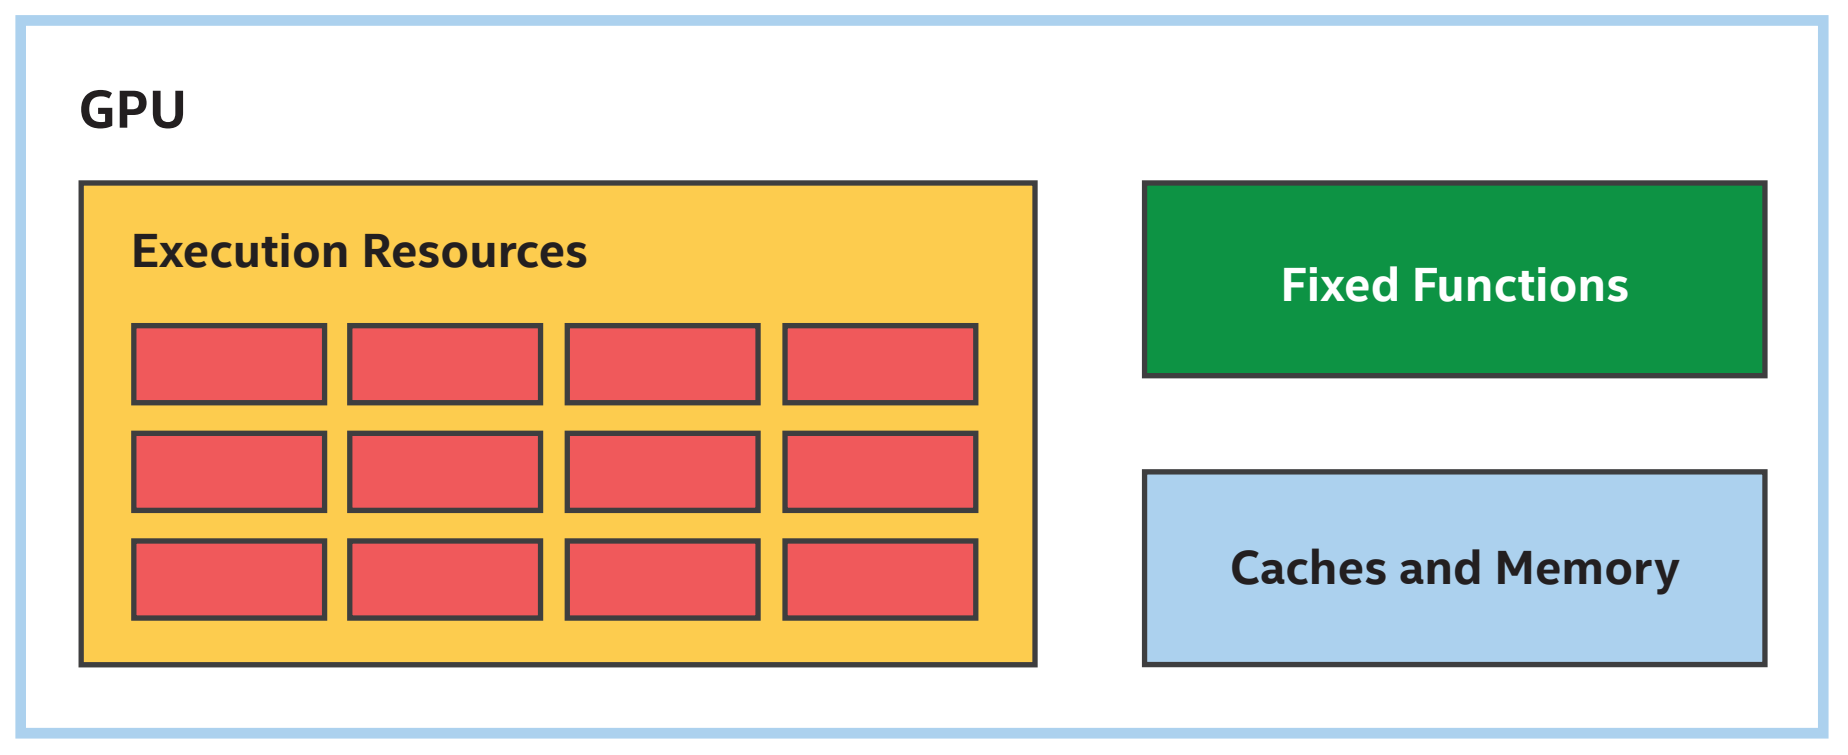
\includegraphics[width=1.0\textwidth]{content/chapter-15/images/2}
\end{center}

\hspace*{\fill} \par %插入空行
\textbf{Simpler Processors (but More of Them)}

Traditionally, when performing graphics operations, GPUs process large batches of data. For example, a typical game frame or rendering workload involves thousands of vertices that produce millions of pixels per frame. To maintain interactive frame rates, these large batches of data must be processed as quickly as possible.\par

A typical GPU design tradeoff is to eliminate features from the processors forming the execution resources that accelerate singlethreaded performance and to use these savings to build additional processors, as shown in Figure 15-2. For example, GPU processors may not include sophisticated out-of-order execution capabilities or branch prediction logic used by other types of processors. Due to these tradeoffs, a single data element may be processed on a GPU slower than it would on another processor, but the larger number of processors enables GPUs to process many data elements quickly and efficiently.\par

\hspace*{\fill} \par %插入空行
Figure 15-2. GPU processors are simpler, but there are more of them
\begin{center}
	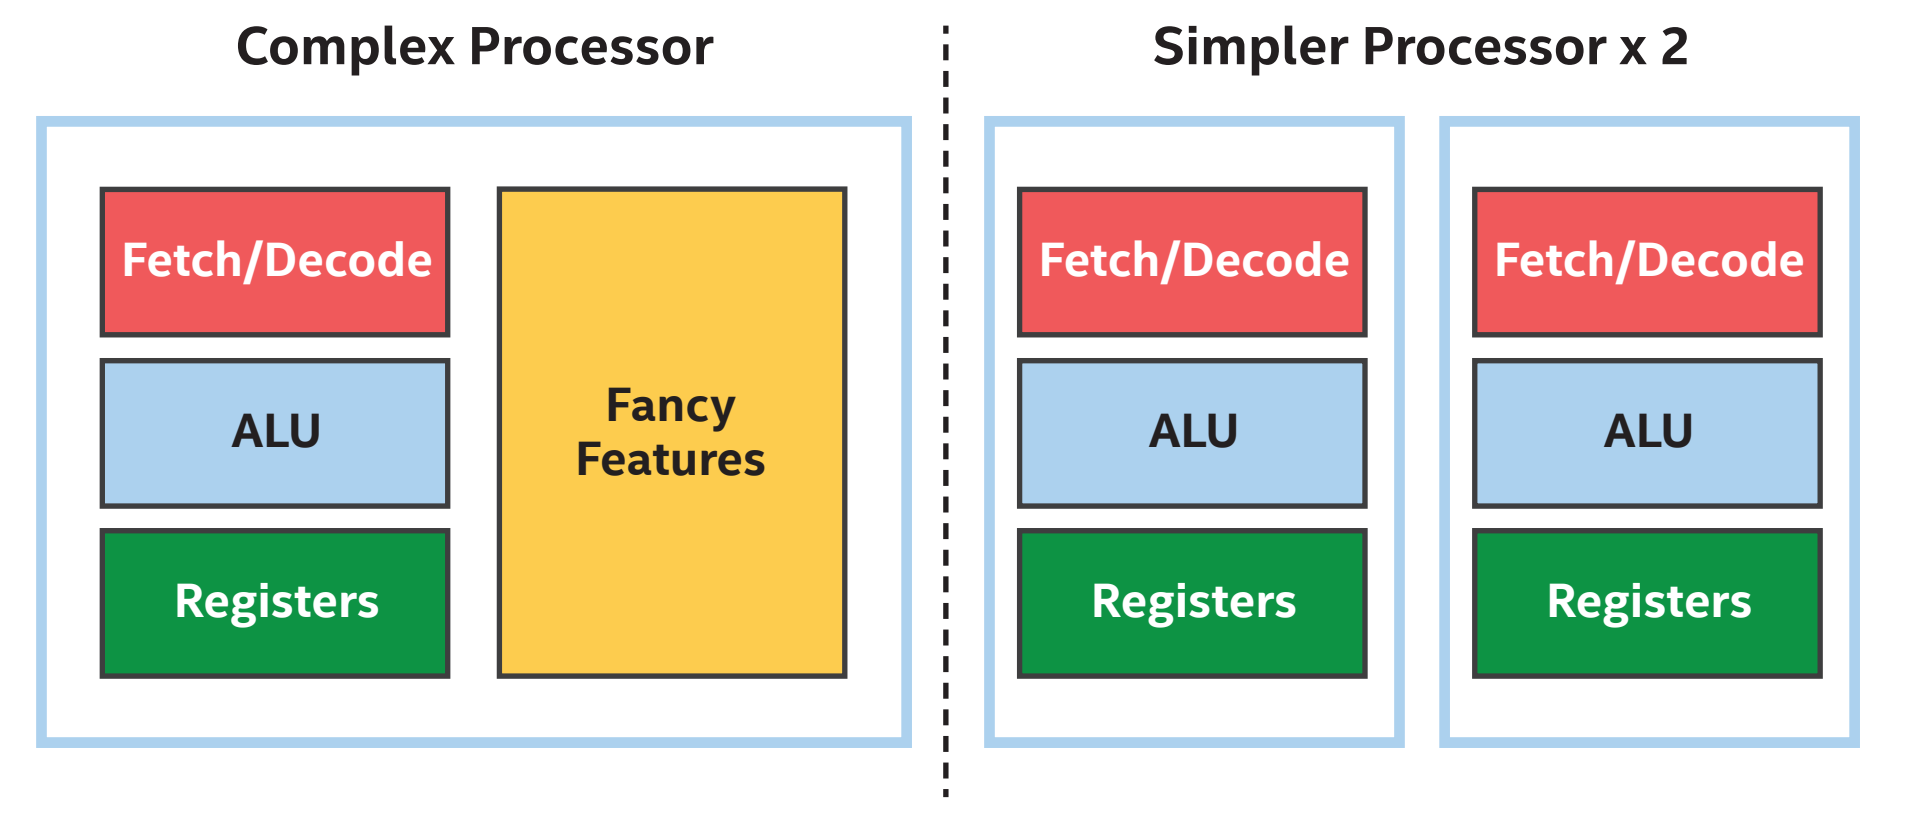
\includegraphics[width=1.0\textwidth]{content/chapter-15/images/3}
\end{center}

To take advantage of this tradeoff when executing kernels, it is important to give the GPU a sufficiently large range of data elements to process. To demonstrate the importance of offloading a large range of data, consider the matrix multiplication kernel we have been developing and modifying throughout this book.\par

\begin{tcolorbox}[colback=blue!5!white,colframe=blue!75!black, title=A REMINDER ABOUT MATRIX MULTIPLICATION]
In this book, matrix multiplication kernels are used to demonstrate how changes in a kernel or the way it is dispatched affects performance. Although matrix multiplication performance are significantly improved using the techniques described in this chapter, matrix multiplication is such an important and common operation that many hardware (GPU, CPU, FPGA, DSP, etc.) vendors have implemented highly tuned versions of many routines including matrix multiplication. Such vendors invest significant time and effort implementing and validating functions for specific devices and in some cases may use functionality or techniques that are difficult or impossible to use in standard kernels.
\end{tcolorbox}

\begin{tcolorbox}[colback=blue!5!white,colframe=blue!75!black, title=USE VENDOR-PROVIDED LIBRARIES!]
When a vendor provides a library implementation of a function, it is almost always beneficial to use it rather than re-implementing the function as a kernel! For matrix multiplication, one can look to oneMKL as part of Intel’s oneAPI toolkits for solutions appropriate for DPC++ programmers.
\end{tcolorbox}

A matrix multiplication kernel may be trivially executed on a GPU by submitting it into a queue as a single task. The body of this matrix multiplication kernel looks exactly like a function that executes on the host CPU and is shown in Figure 15-3.\par

\hspace*{\fill} \par %插入空行
Figure 15-3. A single task matrix multiplication looks a lot like CPU host code
\begin{lstlisting}[caption={}]
h.single_task([=]() {
	for (int m = 0; m < M; m++) {
		for (int n = 0; n < N; n++) {
			T sum = 0;
			for (int k = 0; k < K; k++)
			sum += matrixA[m * K + k] * matrixB[k * N + n];
			matrixC[m * N + n] = sum;
		}
	}
});
\end{lstlisting}

If we try to execute this kernel on a CPU, it will probably perform okay—not great, since it is not expected to utilize any parallel capabilities of the CPU, but potentially good enough for small matrix sizes. As shown in Figure 15-4, if we try to execute this kernel on a GPU, however, it will likely perform very poorly, because the single task will only utilize a single GPU processor.\par

\hspace*{\fill} \par %插入空行
Figure 15-4. A single task kernel on a GPU leaves many execution resources idle
\begin{center}
	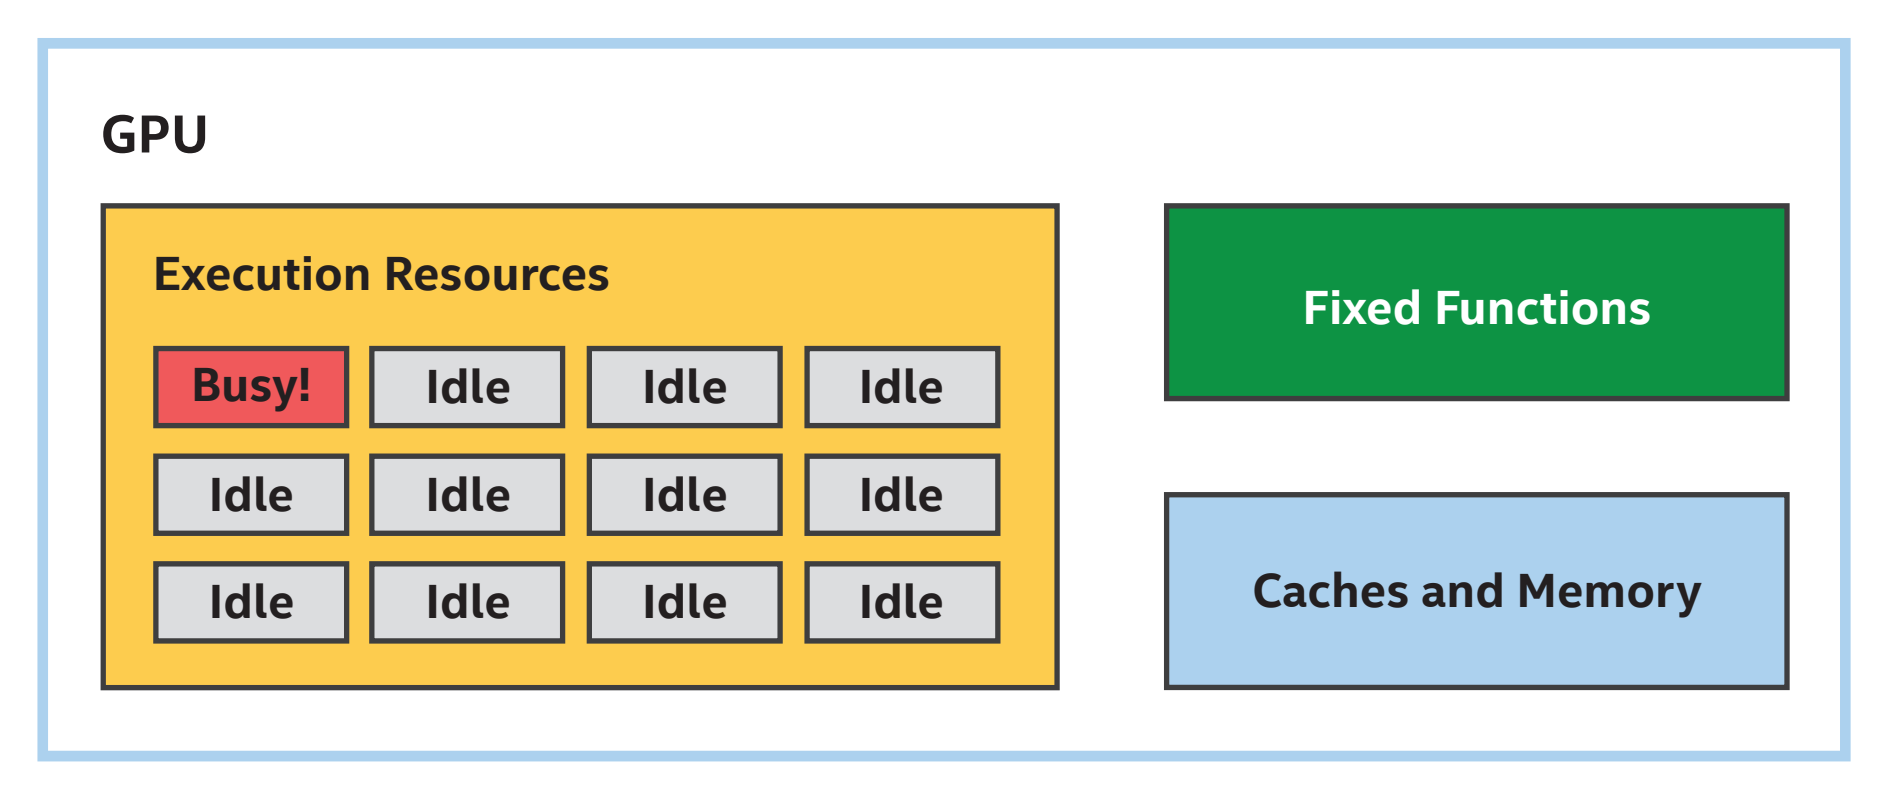
\includegraphics[width=1.0\textwidth]{content/chapter-15/images/4}
\end{center}

\hspace*{\fill} \par %插入空行
\textbf{Expressing Parallelism}

To improve the performance of this kernel for both CPUs and GPUs, we can instead submit a range of data elements to process in parallel, by converting one of the loops to a parallel\_for. For the matrix multiplication kernel, we can choose to submit a range of data elements representing either of the two outermost loops. In Figure 15-5, we’ve chosen to process rows of the result matrix in parallel.\par

\hspace*{\fill} \par %插入空行
Figure 15-5. Somewhat-parallel matrix multiplication
\begin{lstlisting}[caption={}]
h.parallel_for(range{M}, [=](id<1> idx) {
	int m = idx[0];
	for (int n = 0; n < N; n++) {
		T sum = 0;
		for (int k = 0; k < K; k++)
		sum += matrixA[m * K + k] * matrixB[k * N + n];
		matrixC[m * N + n] = sum;
	}
});
\end{lstlisting}

\begin{tcolorbox}[colback=blue!5!white,colframe=blue!75!black, title=CHOOSING HOW TO PARALLELIZE]
Choosing which dimension to parallelize is one very important way to tune an application for both GPUs and other device types. Subsequent sections in this chapter will describe some of the reasons why parallelizing in one dimension may perform better than parallelizing in a different dimension.
\end{tcolorbox}

Even though the somewhat-parallel kernel is very similar to the single task kernel, it should run better on a CPU and much better on a GPU. As shown in Figure 15-6, the parallel\_for enables work-items representing rows of the result matrix to be processed on multiple processor resources in parallel, so all execution resources stay busy.\par

\hspace*{\fill} \par %插入空行
Figure 15-6. Somewhat-parallel kernel keeps more processor resources busy
\begin{center}
	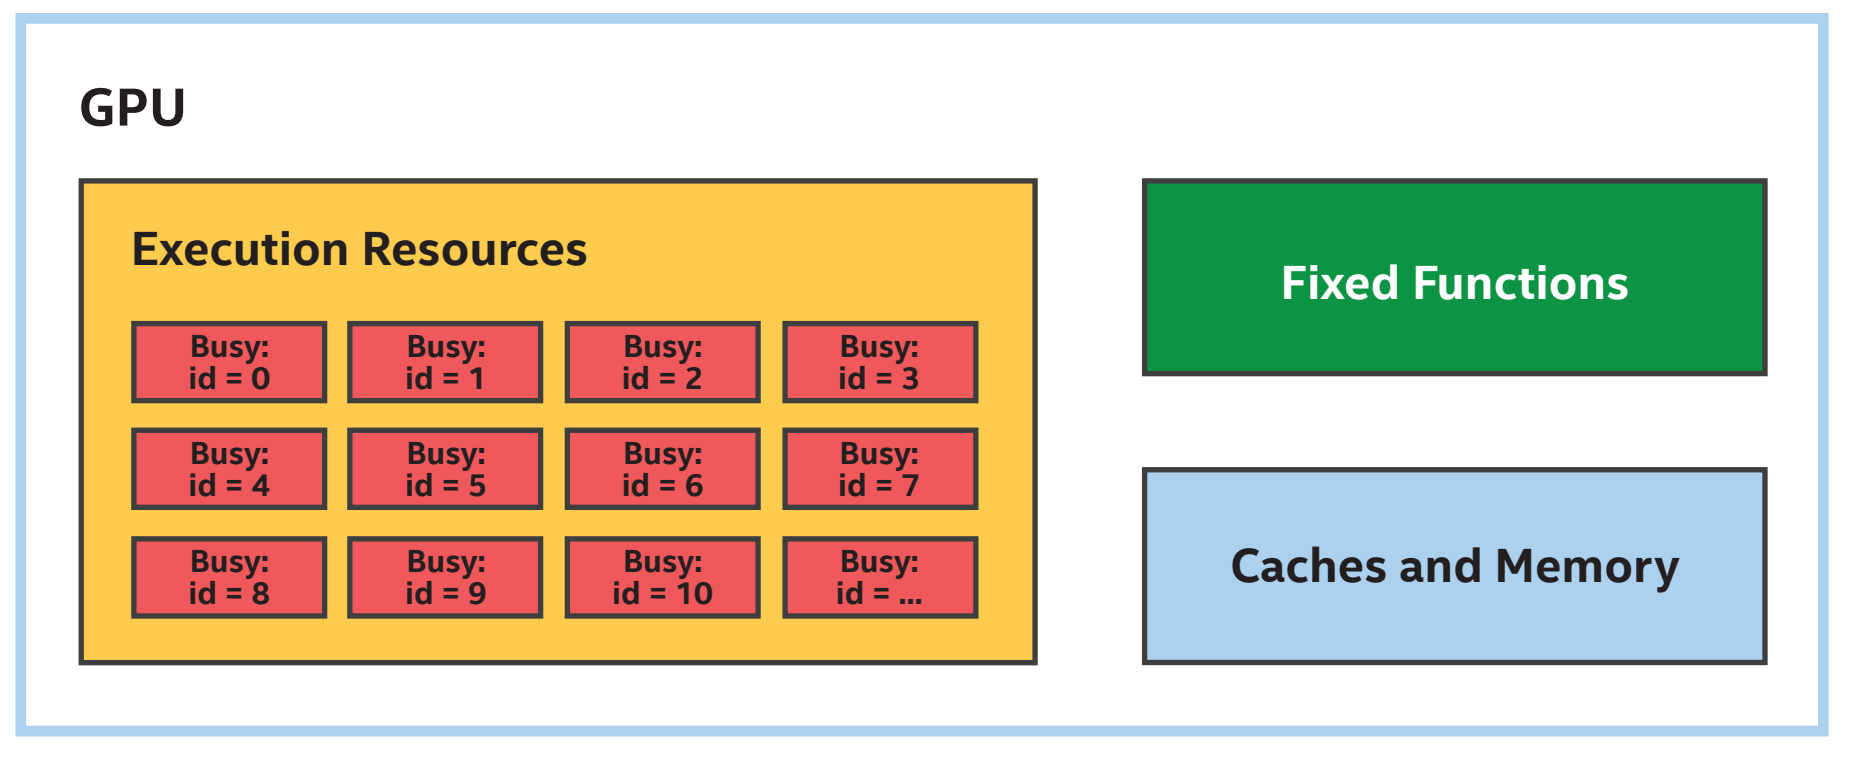
\includegraphics[width=1.0\textwidth]{content/chapter-15/images/5}
\end{center}

Note that the exact way that the rows are partitioned and assigned to different processor resources is not specified, giving an implementation flexibility to choose how best to execute the kernel on a device. For example, instead of executing individual rows on a processor, an implementation may choose to execute consecutive rows on the same processor to gain locality benefits.\par

\hspace*{\fill} \par %插入空行
\textbf{Expressing More Parallelism}

We can parallelize the matrix multiplication kernel even more by choosing to process both outer loops in parallel. Because parallel\_for can express parallel loops over up to three dimensions, this is straightforward, as shown in Figure 15-7. In Figure 15-7, note that both the range passed to parallel\_for and the item representing the index in the parallel execution space are now two-dimensional.\par

\hspace*{\fill} \par %插入空行
Figure 15-7. Even more parallel matrix multiplication
\begin{lstlisting}[caption={}]
h.parallel_for(range{M, N}, [=](id<2> idx) {
	int m = idx[0];
	int n = idx[1];
	T sum = 0;
	for (int k = 0; k < K; k++)
		sum += matrixA[m * K + k] * matrixB[k * N + n];
	matrixC[m * N + n] = sum;
});
\end{lstlisting}

Exposing additional parallelism will likely improve the performance of the matrix multiplication kernel when run on a GPU. This is likely to be true even when the number of matrix rows exceeds the number of GPU processors. The next few sections describe possible reasons why this may be the case.\par

\hspace*{\fill} \par %插入空行
\textbf{Simplified Control Logic (SIMD Instructions)}

Many GPU processors optimize control logic by leveraging the fact that most data elements tend to take the same control flow path through a kernel. For example, in the matrix multiplication kernel, each data element executes the innermost loop the same number of times since the loop bounds are invariant.\par

When data elements take the same control flow path through a kernel, a processor may reduce the costs of managing an instruction stream by sharing control logic among multiple data elements and executing them as a group. One way to do this is to implement a Single Instruction, Multiple Data or SIMD instruction set, where multiple data elements are processed simultaneously by a single instruction.\par

\begin{tcolorbox}[colback=blue!5!white,colframe=blue!75!black, title=THREADS VS. INSTRUCTION STREAMS]
In many parallel programming contexts and GPU literature, the term “thread” is used to mean an “instruction stream.” In these contexts, a “thread” is different than a traditional operating system thread and is typically much more lightweight. This isn’t always the case, though, and in some cases, a “thread” is used to describe something completely different.\\
Since the term “thread” is overloaded and easily misunderstood, this chapter uses the term “instruction stream” instead.
\end{tcolorbox}

\hspace*{\fill} \par %插入空行
Figure 15-8. Four-wide SIMD processor: The four ALUs share fetch/decode logic
\begin{center}
	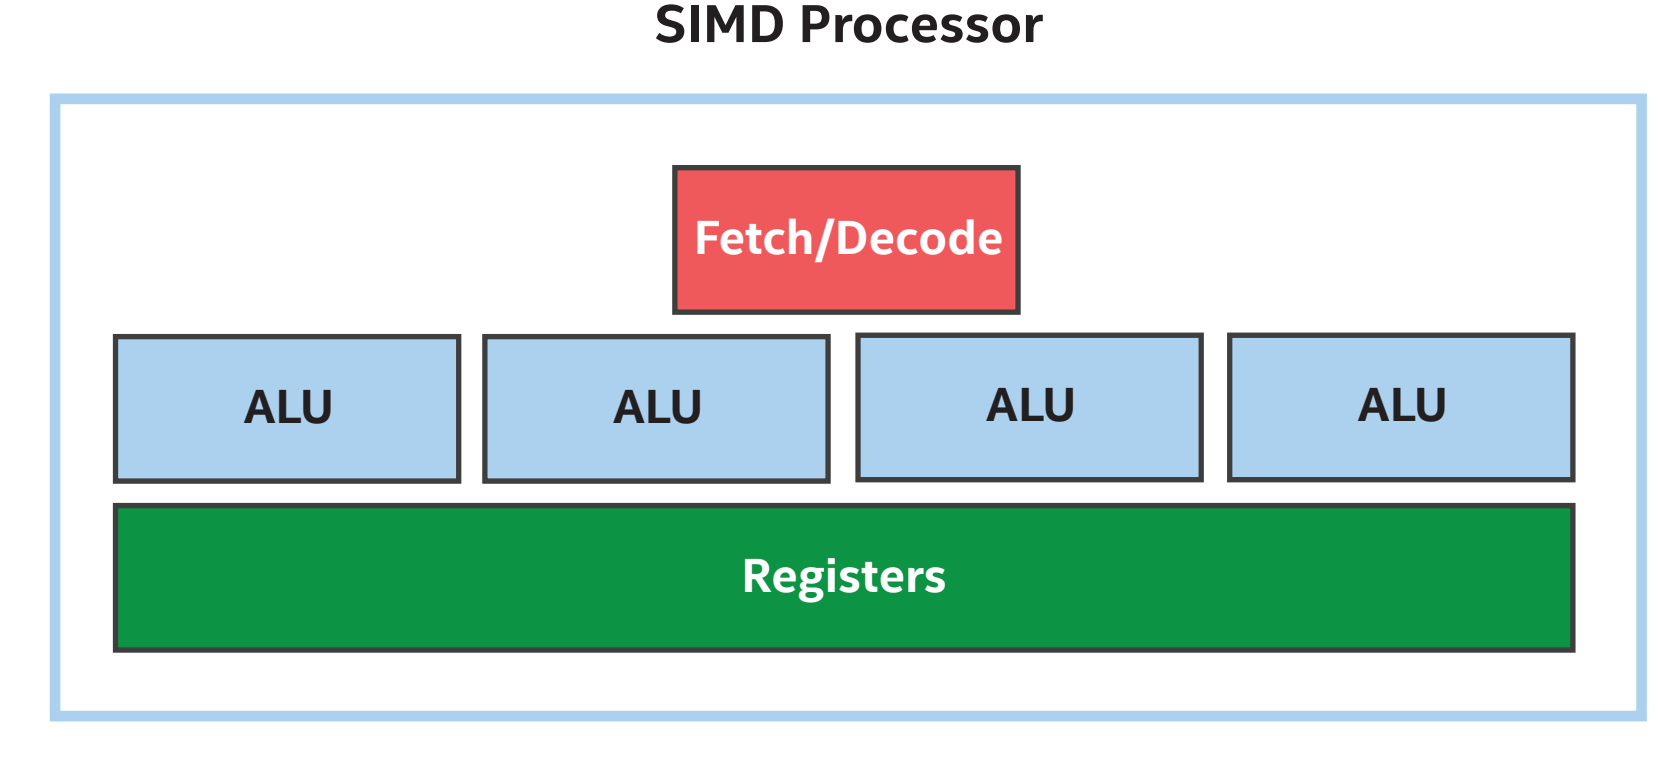
\includegraphics[width=1.0\textwidth]{content/chapter-15/images/6}
\end{center}

The number of data elements that are processed simultaneously by a single instruction is sometimes referred to as the SIMD width of the instruction or the processor executing the instruction. In Figure 15-8, four ALUs share the same control logic, so this may be described as a four-wide SIMD processor.\par

GPU processors are not the only processors that implement SIMD instruction sets. Other processor types also implement SIMD instruction sets to improve efficiency when processing large sets of data. The main difference between GPU processors and other processor types is that GPU processors rely on executing multiple data elements in parallel to achieve good performance and that GPU processors may support wider SIMD widths than other processor types. For example, it is not uncommon for GPU processors to support SIMD widths of 16, 32, or more data elements.\par

\begin{tcolorbox}[colback=blue!5!white,colframe=blue!75!black, title=PROGRAMMING MODELS: SPMD AND SIMD]
Although GPU processors implement SIMD instruction sets with varying widths, this is usually an implementation detail and is transparent to the application executing data-parallel kernels on the GPU processor. This is because many GPU compilers and runtime APIs implement a Single Program, Multiple Data or SPMD programming model, where the GPU compiler and runtime API determine the most efficient group of data elements to process with a SIMD instruction stream, rather than expressing the SIMD instructions explicitly. The “Sub-Groups” section of Chapter 9 explores cases where the grouping of data elements is visible to applications.
\end{tcolorbox}

In Figure 15-9, we have widened each of our execution resources to support four-wide SIMD, allowing us to process four times as many matrix rows in parallel.\par

\hspace*{\fill} \par %插入空行
Figure 15-9. Executing a somewhat-parallel kernel on SIMD processors
\begin{center}
	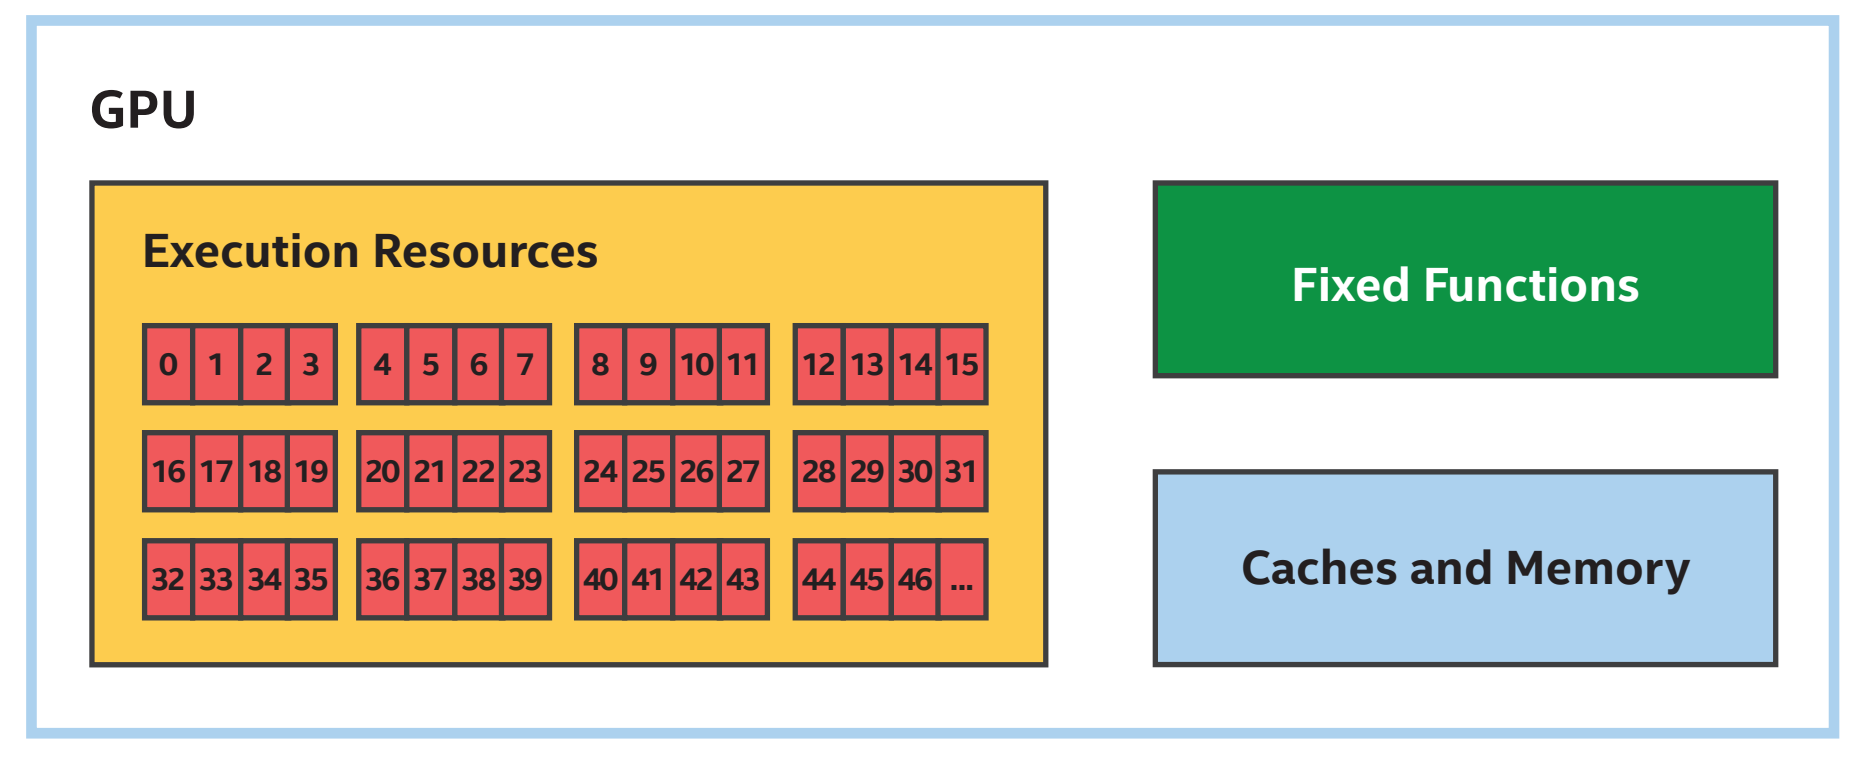
\includegraphics[width=1.0\textwidth]{content/chapter-15/images/7}
\end{center}

The use of SIMD instructions that process multiple data elements in parallel is one of the ways that the performance of the parallel matrix multiplication kernels in Figures 15-5 and 15-7 is able to scale beyond the number of processors alone. The use of SIMD instructions also provides natural locality benefits in many cases, including matrix multiplication, by executing consecutive data elements on the same processor.\par

\begin{tcolorbox}[colback=red!5!white,colframe=red!75!black]
Kernels benefit from parallelism across processors and parallelism within processors!
\end{tcolorbox}

\hspace*{\fill} \par %插入空行
\textbf{Predication and Masking}

Sharing an instruction stream among multiple data elements works well so long as all data elements take the same path through conditional code in a kernel. When data elements take different paths through conditional code, control flow is said to diverge. When control flow diverges in a SIMD instruction stream, usually both control flow paths are executed, with some channels masked off or predicated. This ensures correct behavior, but the correctness comes at a performance cost since channels that are masked do not perform useful work.\par

To show how predication and masking works, consider the kernel in Figure 15-10, which multiplies each data element with an “odd” index by two and increments each data element with an “even” index by one.\par

\hspace*{\fill} \par %插入空行
Figure 15-10. Kernel with divergent control flow
\begin{lstlisting}[caption={}]
h.parallel_for(array_size, [=](id<1> i) {
	auto condition = i[0] & 1;
	if (condition)
		dataAcc[i] = dataAcc[i] * 2; // odd
	else
		dataAcc[i] = dataAcc[i] + 1; // even
});
\end{lstlisting}

Let’s say that we execute this kernel on the four-wide SIMD processor shown in Figure 15-8 and that we execute the first four data elements in one SIMD instruction stream and the next four data elements in a different SIMD instruction stream and so on. Figure 15-11 shows one of the ways channels may be masked and execution may be predicated to correctly execute this kernel with divergent control flow.\par

\hspace*{\fill} \par %插入空行
Figure 15-11. Possible channel masks for a divergent kernel
\begin{center}
	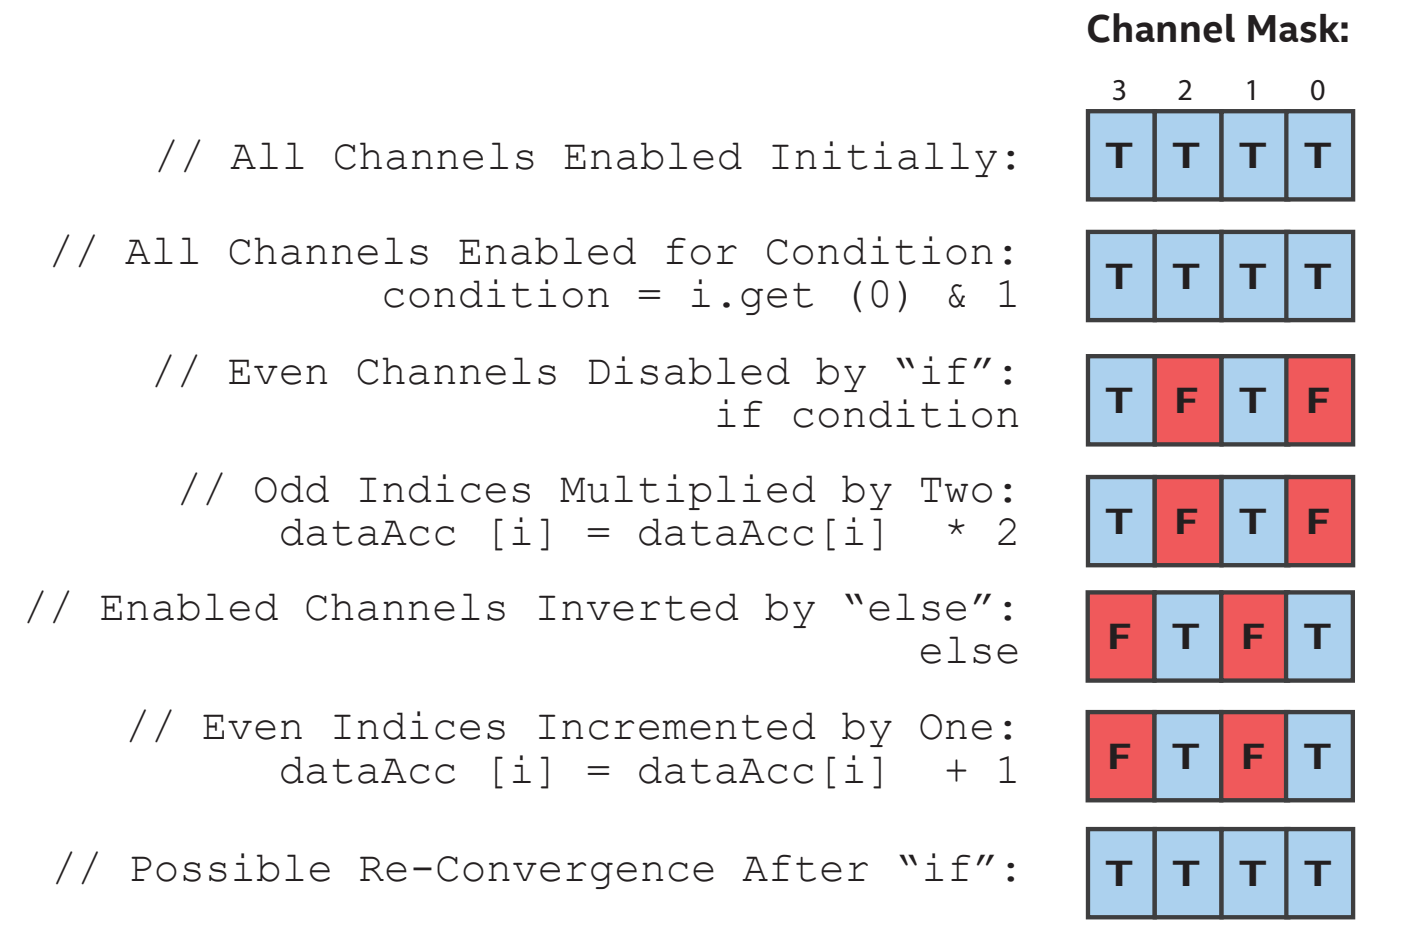
\includegraphics[width=1.0\textwidth]{content/chapter-15/images/8}
\end{center}

\hspace*{\fill} \par %插入空行
\textbf{SIMD Efficiency}

SIMD efficiency measures how well a SIMD instruction stream performs compared to equivalent scalar instruction streams. In Figure 15-11, since control flow partitioned the channels into two equal groups, each instruction in the divergent control flow executes with half efficiency. In a worst-case scenario, for highly divergent kernels, efficiency may be reduced by a factor of the processor’s SIMD width.\par

All processors that implement a SIMD instruction set will suffer from divergence penalties that affect SIMD efficiency, but because GPU processors typically support wider SIMD widths than other processor types, restructuring an algorithm to minimize divergent control flow and maximize converged execution may be especially beneficial when optimizing a kernel for a GPU. This is not always possible, but as an example, choosing to parallelize along a dimension with more converged execution may perform better than parallelizing along a different dimension with highly divergent execution.\par

\hspace*{\fill} \par %插入空行
\textbf{SIMD Efficiency and Groups of Items}

All kernels in this chapter so far have been basic data-parallel kernels that do not specify any grouping of items in the execution range, which gives an implementation freedom to choose the best grouping for a device. For example, a device with a wider SIMD width may prefer a larger grouping, but a device with a narrower SIMD width may be fine with smaller groupings.\par

When a kernel is an ND-range kernel with explicit groupings of workitems, care should be taken to choose an ND-range work-group size that maximizes SIMD efficiency. When a work-group size is not evenly divisible by a processor’s SIMD width, part of the work-group may execute with channels disabled for the entire duration of the kernel. The kernel preferred\_work\_group\_size\_multiple query can be used to choose an efficient work-group size. Please refer to Chapter 12 for more information on how to query properties of a device.\par

Choosing a work-group size consisting of a single work-item will likely perform very poorly since many GPUs will implement a single-work-item work-group by masking off all SIMD channels except for one. For example, the kernel in Figure 15-12 will likely perform much worse than the very similar kernel in Figure 15-5, even though the only significant difference between the two is a change from a basic data-parallel kernel to an inefficient single-work-item ND-range kernel (nd\_range<1>\{M, 1\}).\par

\hspace*{\fill} \par %插入空行
Figure 15-12. Inefficient single-item, somewhat-parallel matrix multiplication
\begin{lstlisting}[caption={}]
// A work-group consisting of a single work-item is inefficient!
h.parallel_for(nd_range<1>{M, 1}, [=](nd_item<1> idx) {
	int m = idx.get_global_id(0);
	
	for (int n = 0; n < N; n++) {
		T sum = 0;
		for (int k = 0; k < K; k++)
			sum += matrixA[m * K + k] * matrixB[k * N + n];
		matrixC[m * N + n] = sum;
	}
});
\end{lstlisting}

\hspace*{\fill} \par %插入空行
\textbf{Switching Work to Hide Latency}

Many GPUs implement one more technique to simplify control logic, maximize execution resources, and improve performance: instead of executing a single instruction stream on a processor, many GPUs allow multiple instruction streams to be resident on a processor simultaneously.\par

Having multiple instruction streams resident on a processor is beneficial because it gives each processor a choice of work to execute. If one instruction stream is performing a long-latency operation, such as a read from memory, the processor can switch to a different instruction stream that is ready to run instead of waiting for the operation to complete. With enough instruction streams, by the time that the processor switches back to the original instruction stream, the long-latency operation may have completed without requiring the processor to wait at all.\par

Figure 15-13 shows how a processor uses multiple simultaneous instruction streams to hide latency and improve performance. Even though the first instruction stream took a little longer to execute with multiple streams, by switching to other instruction streams, the processor was able to find work that was ready to execute and never needed to idly wait for the long operation to complete.\par

\hspace*{\fill} \par %插入空行
Figure 15-13. Switching instruction streams to hide latency
\begin{center}
	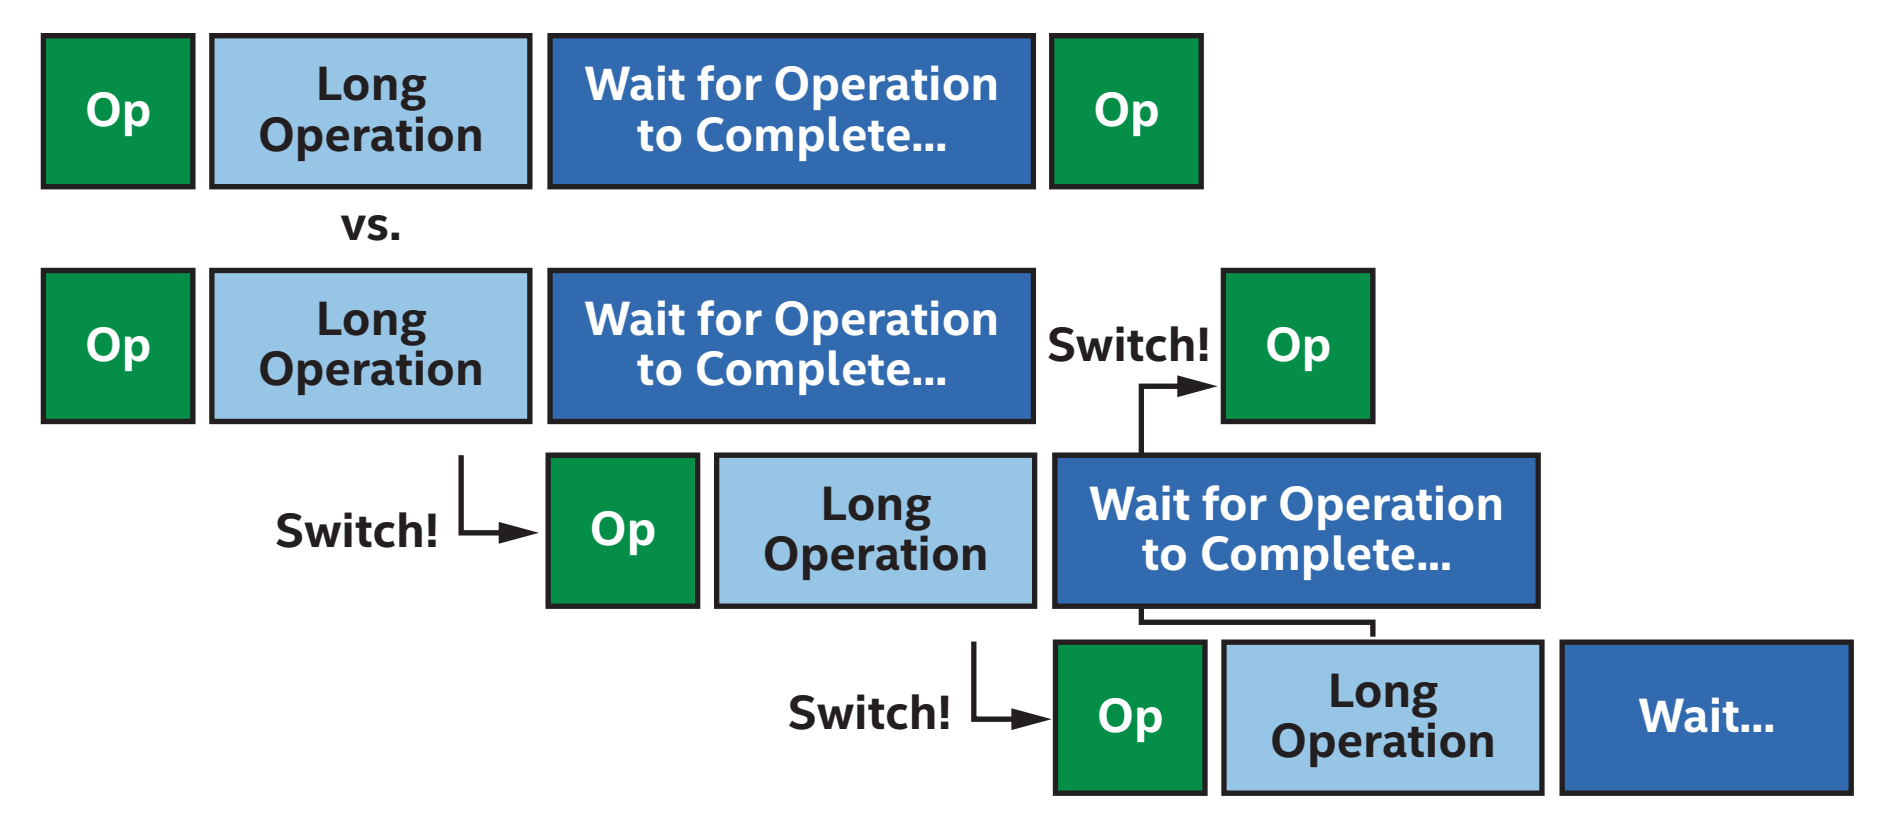
\includegraphics[width=1.0\textwidth]{content/chapter-15/images/9}
\end{center}

GPU profiling tools may describe the number of instruction streams that a GPU processor is currently executing vs. the theoretical total number of instruction streams using a term such as occupancy.\par

Low occupancy does not necessarily imply low performance, since it is possible that a small number of instruction streams will keep a processor busy. Likewise, high occupancy does not necessarily imply high performance, since a GPU processor may still need to wait if all instruction streams perform inefficient, long-latency operations. All else being equal though, increasing occupancy maximizes a GPU processor’s ability to hide latency and will usually improve performance. Increasing occupancy is another reason why performance may improve with the even more parallel 
kernel in Figure 15-7.\par

This technique of switching between multiple instruction streams to hide latency is especially well-suited for GPUs and data-parallel processing. Recall from Figure 15-2 that GPU processors are frequently simpler than other processor types and hence lack complex latency-hiding features. This makes GPU processors more susceptible to latency issues, but because data-parallel programming involves processing a lot of data, GPU processors usually have plenty of instruction streams to execute!\par














